\documentclass[UTF8, aspectratio=169, 10pt]{ctexbeamer}

\usepackage{graphicx}
\usepackage{booktabs}
\usepackage{color}
\usepackage{multirow}
\usepackage{fontspec}
\usepackage{amsmath}
\usepackage{amssymb}
\usepackage{tikz}
\usepackage{subfigure}
\usepackage{amsthm,amsfonts}



% \setmainfont{LMRomanUnsl10-Regular}
% \setmainfont{Noto Sans Mono CJK JP}
\setmainfont{黑体}

% \useoutertheme{miniframes}
\usetheme{Goettingen}
% \usetheme{Madrid}
\title{组会汇报}
\subtitle{基于Game Theory的交互决策}
\author{李鑫}
\institute{吉林大学}
\date{\today}
\begin{document}
\frame{\titlepage}
\frame{\tableofcontents}


\section{背景}
\begin{frame}
 \frametitle{自动驾驶中的决策/规划问题}
\begin{figure}[htbp]
\centering

\subfigure[从A到B问题.]{
\begin{minipage}[t]{0.5\linewidth}
\centering
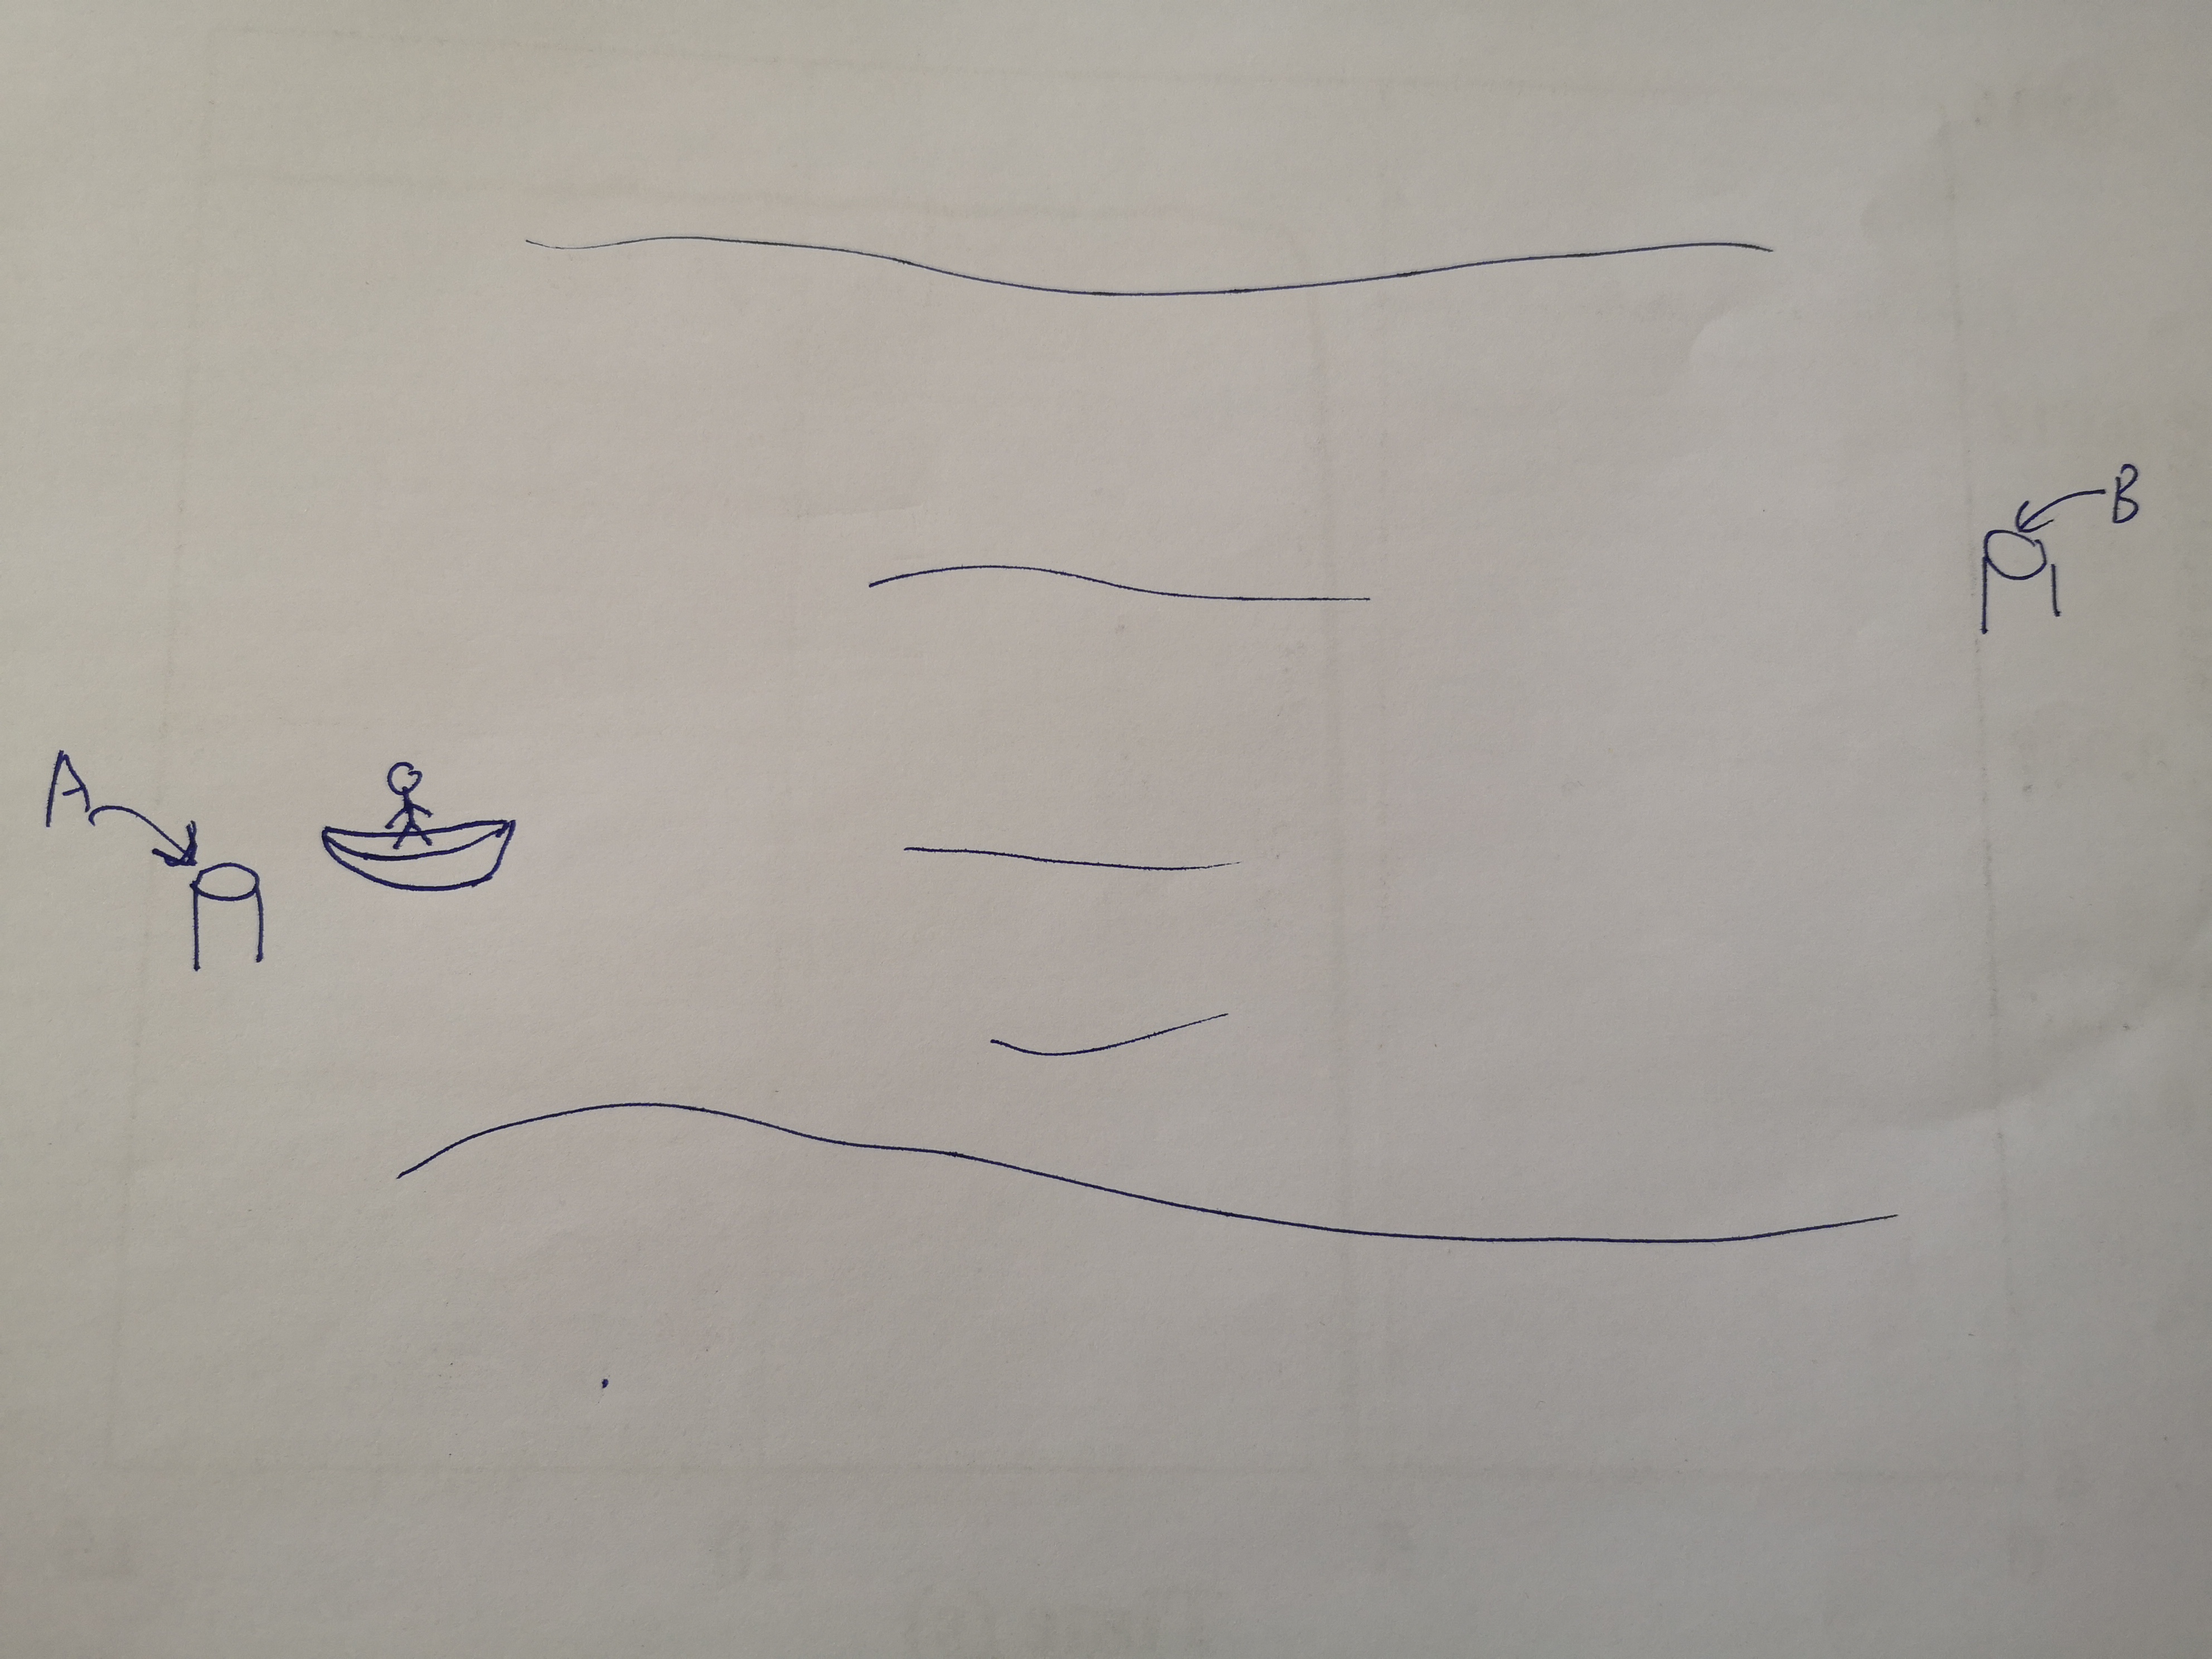
\includegraphics[height=1in,width=2in]{1.jpg}
%\caption{fig1}
\end{minipage}%
}%
\subfigure[从A到B,有静态障碍物的问题.]{
\begin{minipage}[t]{0.5\linewidth}
\centering
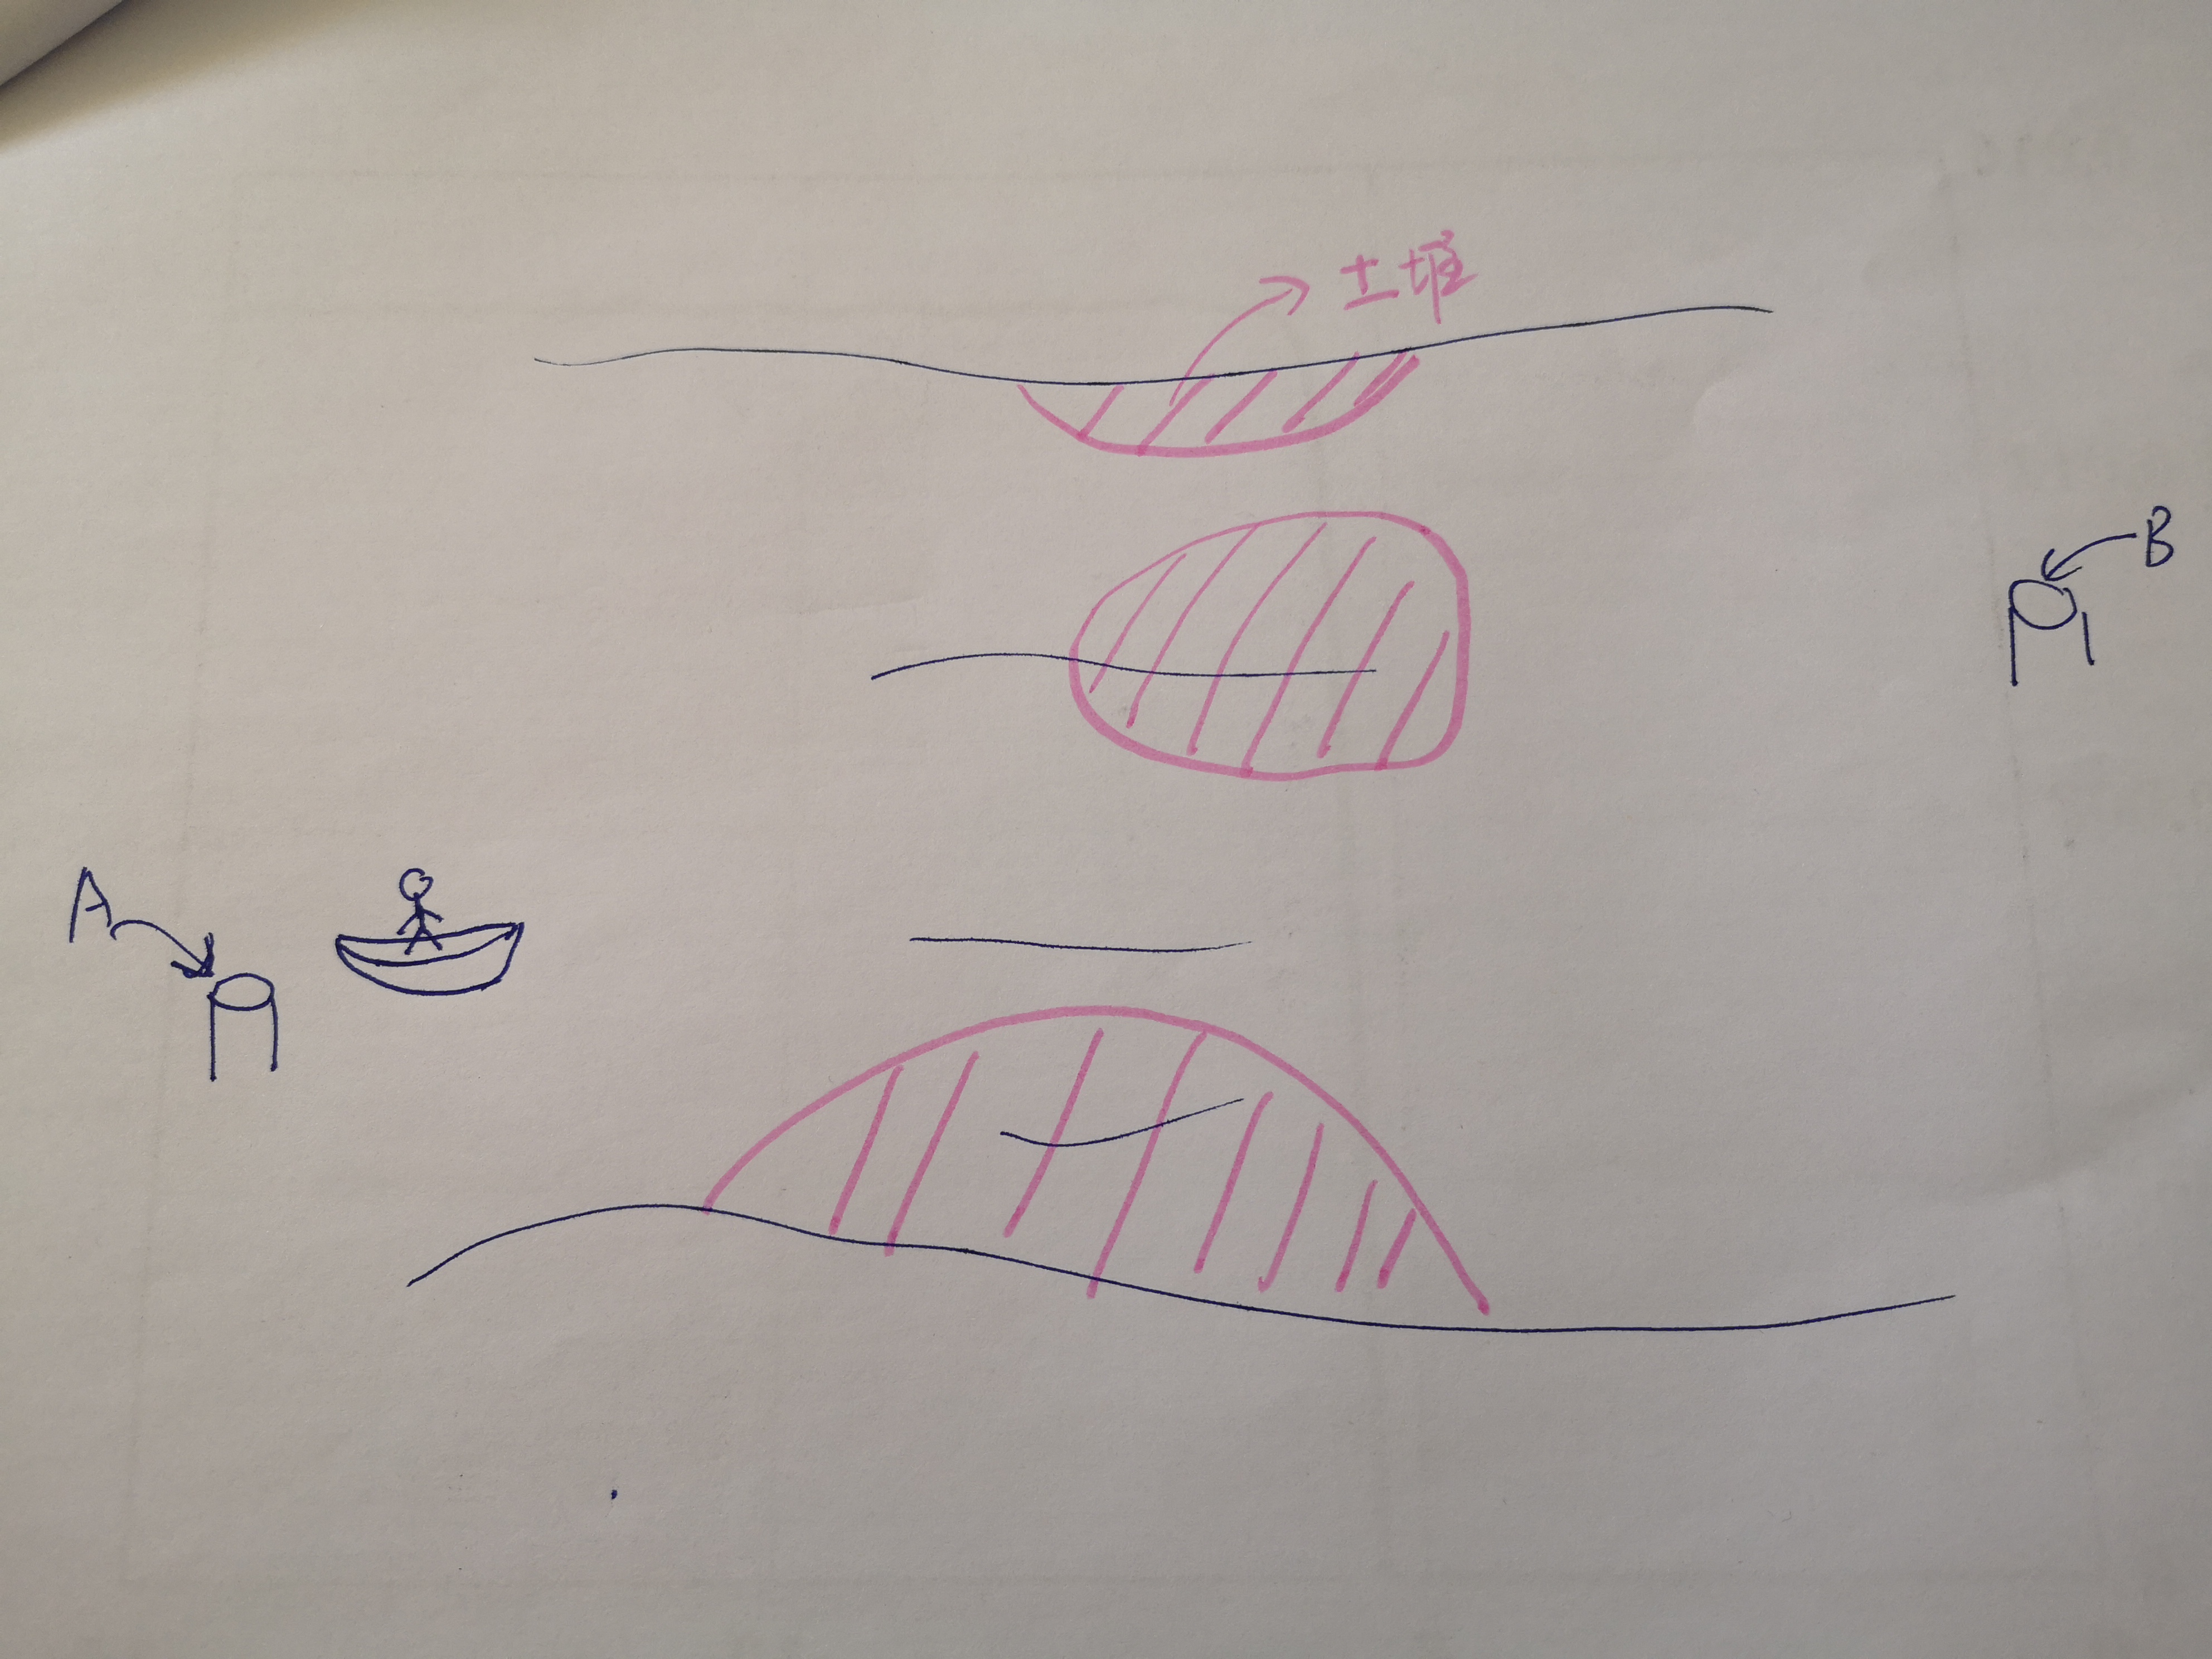
\includegraphics[height=1in,width=2in]{2.jpg}
%\caption{fig2}
\end{minipage}%
}%
        
%这个回车键很重要 \quad也可以
\subfigure[从A到B,有动态障碍物的问题.]{
\begin{minipage}[t]{0.5\linewidth}
\centering
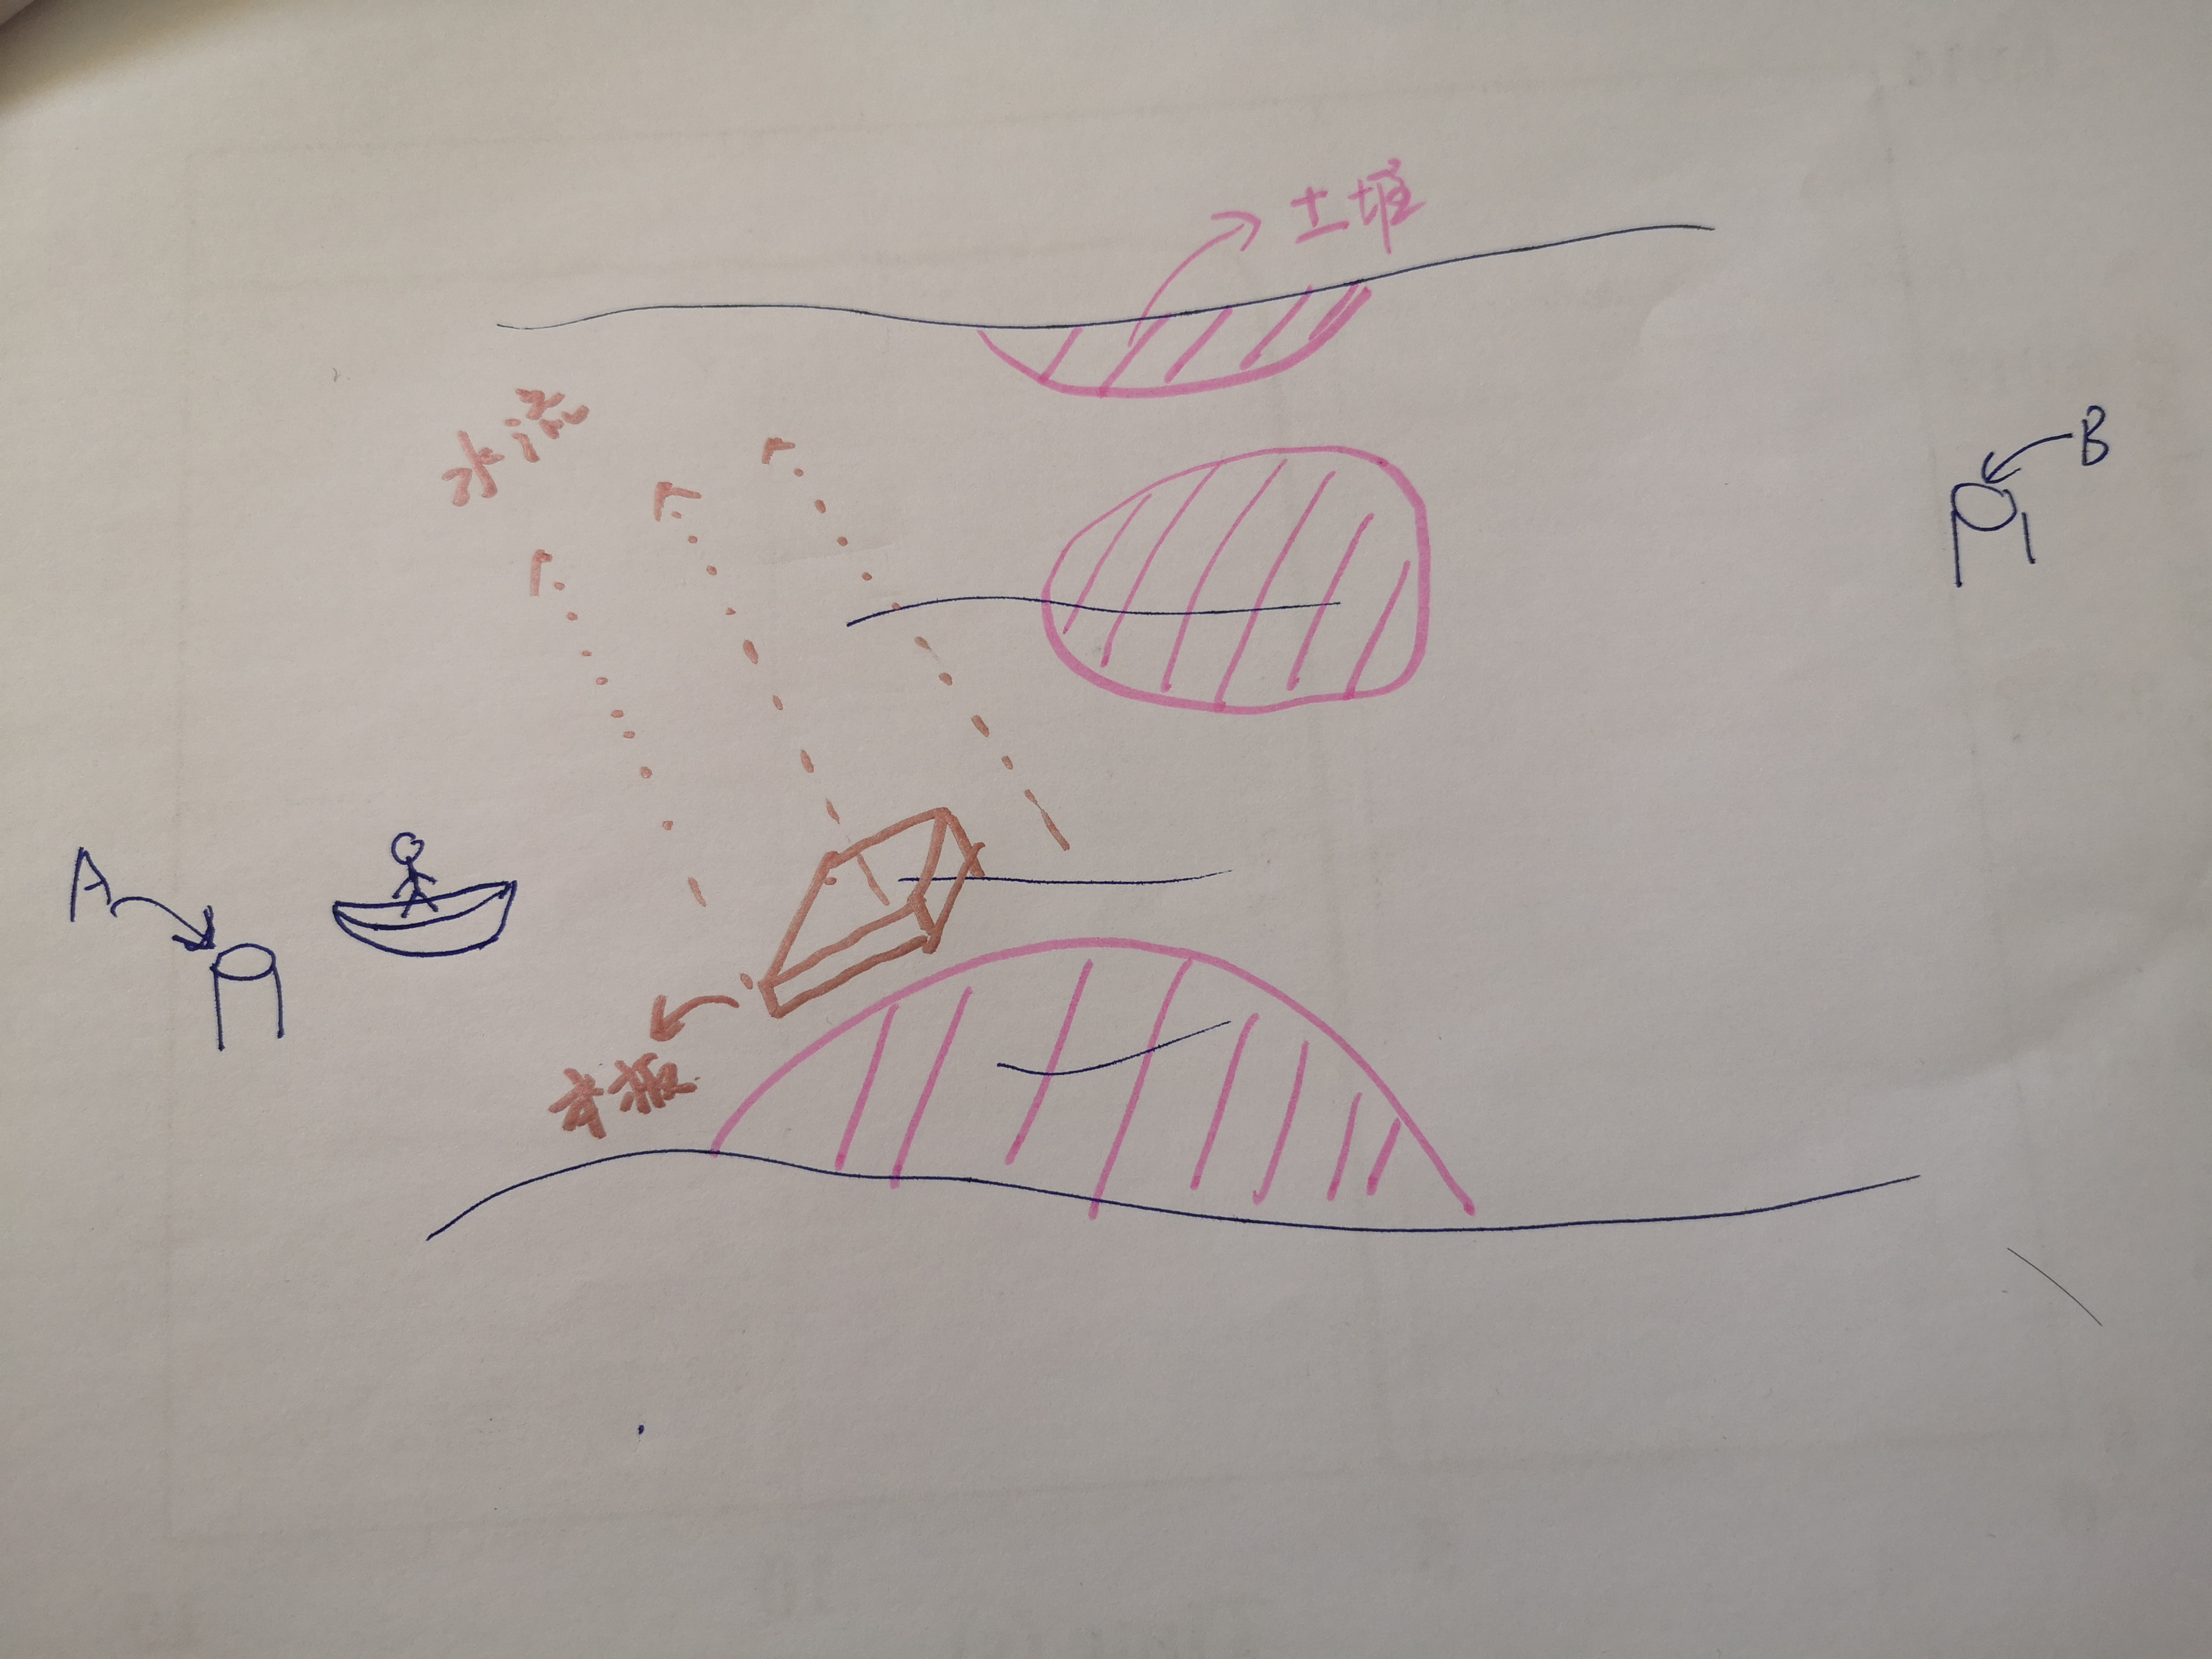
\includegraphics[height=1in,width=2in]{3.jpg}
%\caption{fig2}
\end{minipage}
}%
\subfigure[从A到B,有动态智能体的问题.]{
\begin{minipage}[t]{0.5\linewidth}
\centering
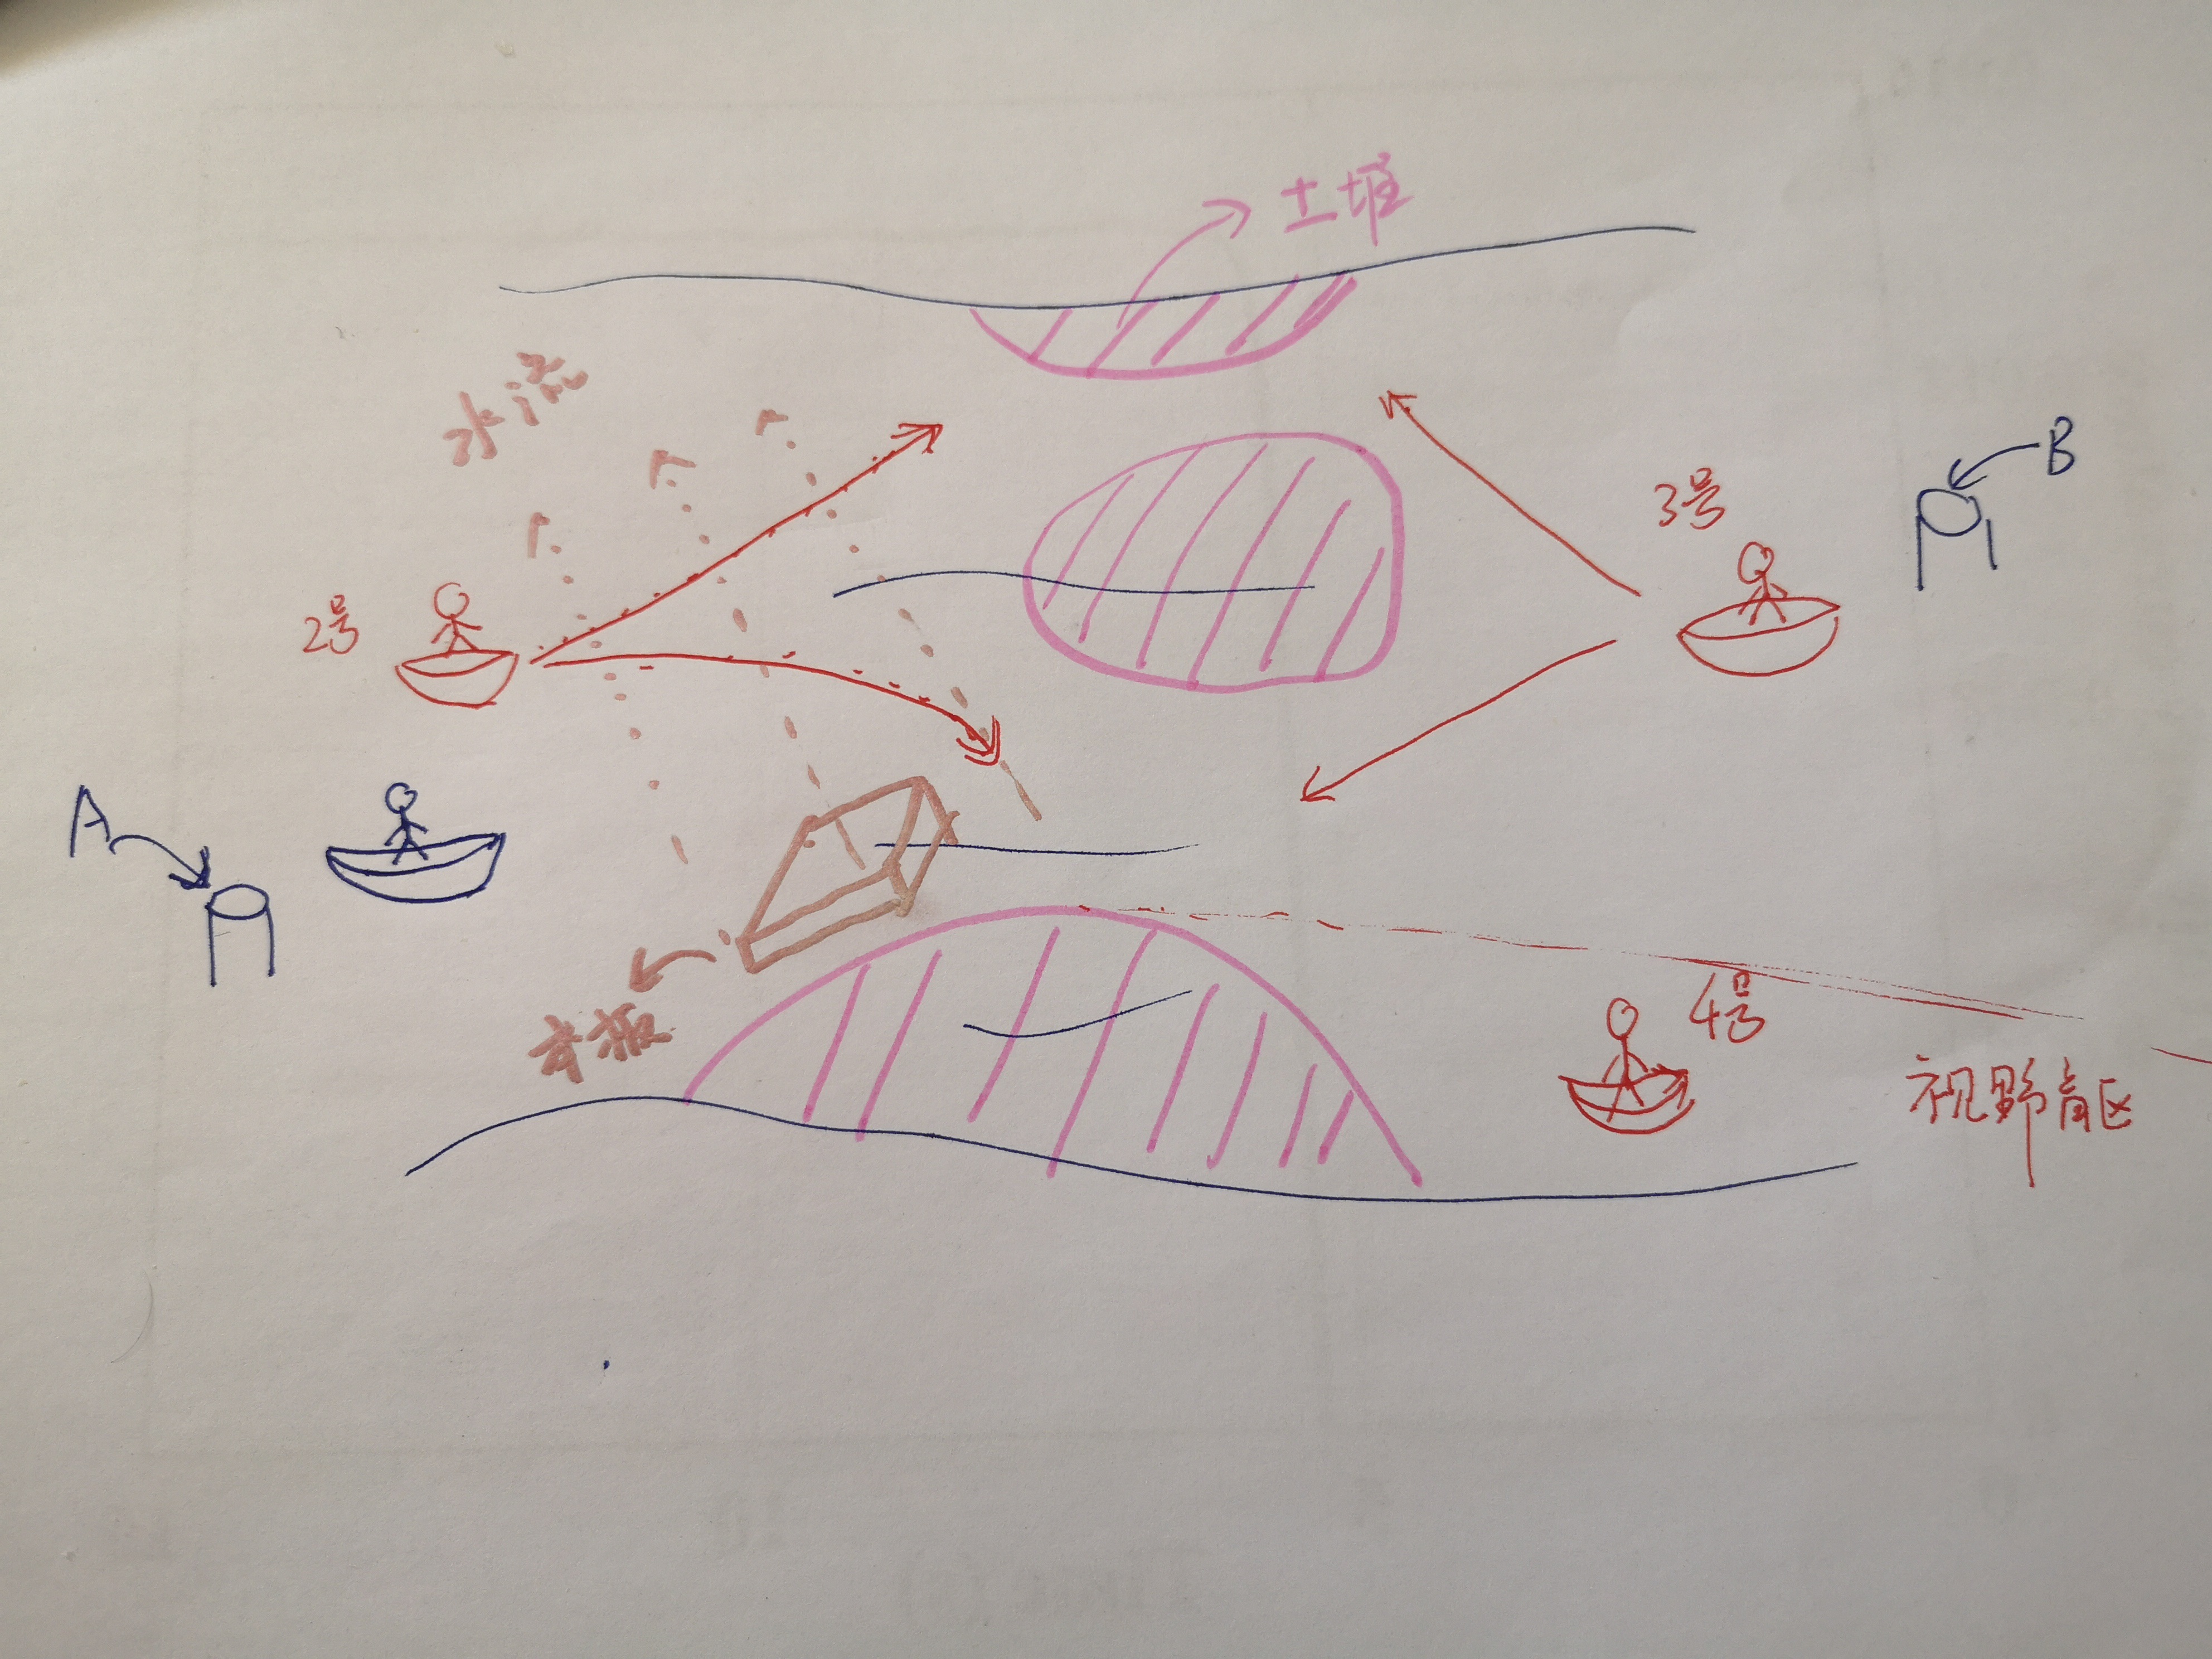
\includegraphics[height=1in,width=2in]{4.jpg}
%\caption{fig2}
\end{minipage}
}%

%\centering
%\caption{ pics}
\end{figure}
\end{frame}


\begin{frame}
  \frametitle{变分法回顾}
  \begin{itemize}
  \item 寻找$f(x)$的局部极小点的必要条件($x_{\min}$)
    \begin{align}
      \frac{dy}{dx} = 0
    \end{align}.
  \item 只能得到驻点/临界点(stationary/critial points),需要进一步验证.
  \item 对于泛函($I[f]$),可以通过类似方法得到Stationary functions of a functional.
  \item 一般而言, 通过需找一个函数 $y=f(x)$ 使得下面的积分:
    \begin{align}
      I[f] = \int_{x_1}^{x_2} F( x, y, \frac{dy}{dx} ) dx
    \end{align}
    stationary.
  \end{itemize}
\end{frame}

\begin{frame}
  \frametitle{Euler-Lagrange 方程推导}
  \begin{itemize}
  \item 假设 $y(x)$ 使得泛函 $I[f]$ stationary 且满足边值条件 $y(x_1) = y_1, \, y(x_2) = y_2$.
  \item 引入辅助函数 $\eta, 满足 \eta (x_1) = \eta (x_2) = 0$.
  \item 构造一个函数 $\bar{y} = \textcolor{red} {y(x)} + \epsilon \eta(x)$ 可以容易得到这个函数和$y(x)$一样满足边值条件,这样构造出来的函数可以表示满足边值条件的函数族.
  \item 在这一族函数里面找特定的函数 $\bar{y} (x)$ 满足泛函stationary的条件,因为构造出来的函数可以通过改变$\epsilon$来改变,所以泛函可以表示为 $I( \epsilon ) =
    \int_{x_1}^{x_2} F( x, \bar{y}, \bar{y}' )$ .
  \item 这样构造出来的泛函只和$\epsilon$有关,变成了一维问题, 所以一阶条件变成了
    $\frac{dI}{d \epsilon} |_{\epsilon = 0} = 0$,

    \begin{align}
      \begin{split}
        & \frac{d}{d \epsilon} |_{\epsilon = 0} \, \int_{x_1}^{x_2} F(x,
        \bar{y}, \bar{y}' ) dx = 0 \Rightarrow \int_{x_1}^{x_2}
        \frac{\partial}{\partial
          \epsilon} F( x, \bar{y}, \bar{y}' ) |_{\epsilon} dx = 0 \\
        \Rightarrow & \int_{x_1}^{x_2} \big [ \frac{ \partial F }{ \partial
          \bar{y} } \frac{ \partial \bar{y} }{ \partial \epsilon } + \frac{
          \partial F }{ \partial \bar{y}' } \frac{ \partial \bar{y}' }{ \partial
          \epsilon } \big ] |_{\epsilon=0} dx = 0
        \Rightarrow  \int_{x_1}^{x_2} \big [ \frac{ \partial F }{ \partial
          \bar{y} } \eta (x) + \frac{
          \partial F }{ \partial \bar{y}' } \textcolor {blue} {\eta'(x)} \big ] |_{\epsilon=0} dx =
        0 \\
        \Rightarrow & \int_{x_1}^{x_2} \big [ \frac{ \partial F }{ \partial
          \bar{y} } \eta (x) - \frac{d}{dx} \big ( \frac{
          \partial F }{ \partial \bar{y}' } \big ) \eta(x) \big ] |_{\epsilon=0} dx =
        0
        \Rightarrow  \int_{x_1}^{x_2} \big [ \frac{ \partial F }{ \partial
          \bar{y} }  - \frac{d}{dx} \big ( \frac{
          \partial F }{ \partial \bar{y}' } \big )  \big ] \eta(x) |_{\textcolor
          {red} {\epsilon=0} } dx =
        0  \\
        \Rightarrow & \int_{x_1}^{x_2} \big [ \frac{ \partial F }{ \partial
          \textcolor {red} {y} }  - \frac{d}{dx} \big ( \frac{
          \partial F }{ \partial \textcolor {red} {y} } \big )  \big ] \eta(x)  dx =
        0
        \Rightarrow \textcolor[rgb]{1.00,0.00,0.00}{ \frac{ \partial F }{ \partial
          {y} }  - \frac{d}{dx} \big ( \frac{
          \partial F }{ \partial  {y} } \big )  = 0 }
      \end{split}
    \end{align}.

  \end{itemize}
\end{frame}


\begin{frame}
  \frametitle{庞特里亚金极大值原理}
  \begin{itemize}
    \item 一般优化控制问题
    \begin{align}
      \begin{split}
\max  \, & \int_{0}^{T} L(t, x(t), u(t)) \mathrm{d} t+\Psi(T, x(T)) \\
 \text { s.t. } & \dot{x}(t)=f(t, x(t), u(t)), \quad \text { a.e. } t \in[0, T] \\
& x(0)=x_{0} \\
& (T, x(T)) \in \mathcal{T} \subseteq \mathbb{R}^{n+1} \\
& u(t) \in U \subseteq \mathbb{R}^{m}, \quad \text { a.e. } t \in[0, T]
\end{split}
    \end{align}
    \item Bolza form
    $$ \int_{0}^{T} L(t, x(t), u(t)) \mathrm{d} t+\Psi(T, x(T)) $$
    \item Lagrange form
    $$ \int_{0}^{T} L(t, x(t), u(t)) \mathrm{d} t
    $$
    \item Mayer form
    $$ \Psi(T, x(T))
    $$ 
  \end{itemize}
\end{frame}

\begin{frame}
\frametitle{没有终端约束的PMP推导 }
拉格朗日形式
$$
  \mathcal{L}(x, u, p):=\Psi(x(T))+\int_{0}^{T} p(t)(f(t, x(t), u(t))-\dot{x}(t)) \mathrm{d} t,
$$
对$x$求偏导
$$
D_{x} \mathcal{L}(x, u, p) z=\nabla \Psi(x(T)) z(T)+\int_{0}^{T} p(t)\left(D_{x} f(t, x(t), u(t)) z(t)-\dot{z}(t)\right) \mathrm{d} t
$$
分部积分得到
\begin{align*}
  \begin{split}
  D_{x} \mathcal{L}(x, u, p) z=&(\underbrace{\nabla \Psi(x(T))-p(T)}_{\text {终端条件 } p}) z(T)+p(0) \underbrace{z_{0}}_{=0} \\
&+\int_{0}^{T}(\underbrace{p(t) D_{x} f(t, x(t), u(t))+\dot{p}(t)}_{\text {动态条件 } p}) z(t) \mathrm{d} t
  \end{split}
\end{align*}
\end{frame}



\begin{frame}
\frametitle{没有终端约束的PMP推导 }
\begin{theorem}
  设$u^*$ 是最优控制,$x^*$是相应的状态轨迹,$p:[0,T] \rightarrow \mathbb{R}^{n,*}$是adjoint equation的解
  $$
  \dot{p}(t)=-p(t) D_{x} f\left(t, x^{*}(t), u^{*}(t)\right),
  $$
  同时满足
  $$
  p(T)=\nabla \Psi\left(x^{*}(T)\right).
  $$
  则,PMP最大值原理条件为
  $$
  p(t) f\left(t, x^{*}(t), u^{*}(t)\right)=\max _{\omega \in U} p(t) f\left(t, x^{*}(t), \omega\right), \quad \text { a.e. } \quad t \in[0, T]
  $$
\end{theorem}
定义 Hamiltonian 为$H(t, x, u, p):=p f(t, x, u)$,那么PMP就是在说满足
$
\dot{p}(t)=-D_{x} H\left(t, x^{*}(t), u^{*}(t), p(t)\right), \quad p(T)=\nabla \Psi\left(x^{*}(T)\right)
$
最大值条件为
$$H\left(t, x^{*}(t), u^{*}(t), p(t)\right)=\max _{\omega \in U} H\left(t, x^{*}(t), \omega, p(t)\right), \quad \text { a.e. } \quad t \in[0, T]
$$
\end{frame}

\begin{frame}
\begin{proof}
  a
\end{proof}
\end{frame}

\begin{frame}
  \frametitle{IQR回顾}

  \begin{itemize}
  \item 系统方程,线性系统
    \begin{align}
      \dot{ \boldsymbol{ x } } = \boldsymbol{ A x } + \boldsymbol{ B u }, \quad
      \boldsymbol{x}_0 = \boldsymbol{x}(0)
    \end{align}

  \item 代价函数
    \begin{align}
      J(\boldsymbol{x}, x_0) = \frac{1}{2} \boldsymbol{x}^T_T \boldsymbol{S}
      \boldsymbol{ x }_T + \frac{1}{2} \int_0^T \boldsymbol{x}^T_t
      \boldsymbol{Q} \boldsymbol{x}_t + \boldsymbol{u}^T_t \boldsymbol{R}
      \boldsymbol{u}_t dt
    \end{align}.

  \item 问题转换为
    \begin{align}
      J( \boldsymbol{u}^{*}, \boldsymbol{x}_0 ) = \underset{ \boldsymbol{u}
      }{min}  \, J(
      \boldsymbol{u}, \boldsymbol{x}_0 )
    \end{align}.

  \item 动态规划
    \begin{align}
       J( \boldsymbol{u}, \boldsymbol{x}_0 ) = \phi( \boldsymbol{x}_{T} ) + \int_0^T
      \Phi( \boldsymbol{x}_t,  \boldsymbol{u}_t, t ) dt
    \end{align}.

  \end{itemize}
\end{frame}

\begin{frame}
  \frametitle{IQR回顾}
  \begin{itemize}
    \item 定义$t$时刻的值函数,衡量从$t$时刻$\boldsymbol{x}_t$到$T$时刻
      $\boldsymbol{x}_T$在最佳控制下,成本的大小

      \begin{align}
        \begin{split}
      V( \boldsymbol{x}_t, t )   &=
      \underset{ \boldsymbol{u} }{min} \,
      \big \{
      \int_t^T\Phi( \boldsymbol{x}_t,  \boldsymbol{u}_t, t ) dt + \phi( \boldsymbol{x}_{T} )
      \big \} \\
      &= \underset{u}{min} \, J(\boldsymbol{u}, \boldsymbol{x}_t ) \\
      &= J(\boldsymbol{u}^{*}, \boldsymbol{x}_t )
      \end{split}
    \end{align}.

  \item 在$[t,T]$之间选择任意一个时刻$t'$,则
    \begin{align}
      \label{optim}
      \begin{split}
        V( \boldsymbol{x}_t, t )
        =&
      \underset{ \boldsymbol{u} }{min} \,
      \big \{
      \int_t^{t'}\Phi( \boldsymbol{x}_t,  \boldsymbol{u}_t, t ) dt  +
      \int_{t'}^{T}\Phi( \boldsymbol{x}_t,  \boldsymbol{u}_t, t ) dt  +
      \phi( \boldsymbol{x}_{T} )
      \big \} \\
      \overset{ \textcolor{red} {  最优性原则 } }{=}&
      \underset{ \boldsymbol{u} }{min} \,
      \big \{
      \int_t^{t'}\Phi( \boldsymbol{x}_t,  \boldsymbol{u}_t, t ) dt  +
      V( \boldsymbol{x}_{t'}, t' )
      \big \}
      \end{split}
    \end{align}

  \end{itemize}

\end{frame}

\begin{frame}
  \frametitle{IQR回顾}
  \begin{itemize}
  \item $V( \boldsymbol{x}_{t'}, t' )$ 泰勒展开
    \begin{align}
      V( \boldsymbol{x}_{t'}, t' ) = V( \boldsymbol{x}_{t}, t ) + \frac{
      \partial V^T ( \boldsymbol{x}, t  ) } { \partial
      \boldsymbol{x}  } \, \dot { \boldsymbol{x} }  \Delta t + \frac{ \partial V
      ( \boldsymbol{x}, t )}{ \partial t } \Delta t + \mathcal{O} ( \Delta t^2 )
    \end{align}.
  \item $      \int_t^{t'}\Phi( \boldsymbol{x}_t,  \boldsymbol{u}_t, t ) dt$ 泰
    勒展开
    \begin{align}
            \int_t^{t'}\Phi( \boldsymbol{x}_t,  \boldsymbol{u}_t, t ) dt = \Phi(
      \boldsymbol{x}_t,  \boldsymbol{u}_t, t ) \Delta t + \mathcal{O} (\Delta
      t^2 )
    \end{align}.
  \item 带入公式 (\ref{optim})得
    \begin{align}
      V( \boldsymbol{x}, t ) = \underset{u}{min} \big \{
      \Phi(
      \boldsymbol{x}_t,  \boldsymbol{u}_t, t ) \Delta t + \textcolor{blue} { V(
      \boldsymbol{x}_{t}, t ) } + \frac{
      \partial V^T ( \boldsymbol{x}, t  ) } { \partial
      \boldsymbol{x}  } \, \dot { \boldsymbol{x} }  \Delta t + \textcolor{blue} { \frac{ \partial V
      ( \boldsymbol{x}, t )}{ \partial t } } \Delta t
      + \mathcal{O} (\Delta
      t^2 )
      \big \}
    \end{align}.
  \item 对于上面公式,蓝色的和$u$无关,提出来化简得到
    \begin{align}
      \label{hjb}
      0 = \textcolor{blue} { \frac{ \partial V
      ( \boldsymbol{x}, t )}{ \partial t } }  +
      \underset{u}{min} \big \{
      \Phi(
      \boldsymbol{x}_t,  \boldsymbol{u}_t, t )  + \frac{
      \partial V^T ( \boldsymbol{x}, t  ) } { \partial
      \boldsymbol{x}  } \, f(\boldsymbol{x}, \boldsymbol{u}, t)
      \big \}
    \end{align}.

  \end{itemize}
\end{frame}

\begin{frame}
  \frametitle{LQR回顾}
  \begin{itemize}
  \item 如果是线性方程且性能指标为二次
    \begin{align}
      \begin{split}
        f( \boldsymbol{x}, \boldsymbol{u}, t ) = \boldsymbol{A x} +
        \boldsymbol{B u} \\
        \int_0^T \Phi ( \boldsymbol{x}_t,  \boldsymbol{u}_t, t ) dt  =
        \frac{1}{2} \int_0^T \boldsymbol{x}^T_t \boldsymbol{Q} \boldsymbol{x}_t
        + \boldsymbol{u}^T_t \boldsymbol{R} \boldsymbol{u}_t dt
      \end{split}
    \end{align}.
  \item 公式(\ref{hjb}) 为
      \begin{align}
      \label{linear-hjb}
      0 = \textcolor{blue} { \frac{ \partial V
      ( \boldsymbol{x}, t )}{ \partial t } }  +
      \underset{u}{min} \big \{
        \frac{1}{2}  \boldsymbol{x}^T_t \boldsymbol{Q} \boldsymbol{x}_t
        + \frac{1}{2} \boldsymbol{u}^T_t \boldsymbol{R} \boldsymbol{u}_t
        + \frac{
      \partial V^T ( \boldsymbol{x}, t  ) } { \partial
      \boldsymbol{x}  } \, ( \boldsymbol{A x} +
        \boldsymbol{B u} )
      \big \}
    \end{align}.

  \end{itemize}
\end{frame}

\begin{frame}
  \frametitle{交互式决策如何做}
  \begin{itemize}
  \item 把其他智能体当作一个扰动-鲁棒控制.
  \item 把其他智能体的动作考虑到模型-博弈理论.
  \item 基于数据的-MARL.
  \end{itemize}
\end{frame}

\begin{frame}
  \frametitle{简单的连续博弈控制问题}
  \begin{itemize}
  \item 两辆车一追一逃,以相互距离为性能指标.
  \item 在系统中,状态的变换和性质指标都是由二者共同决定.
  \item $x_1^i$表示第$i$个智能体的位置,$x_2^i$表示第$i$个智能体的速度.
  \item $u^{(i)}$表示第$i$个智能体的加速度.
  \item 数学表达
    \begin{align}
      \left\{\begin{matrix}
          \dot{x}_1^{(1)} (t) = x_2^{(1)} (t), \\
          \dot{x}_2^{(1)} (t) = u^{(1)} (t). \\
        \end{matrix}\right.
      \quad \quad \quad
      \left\{\begin{matrix}
          \dot{x}_1^{(2)} (t) = x_2^{(2)} (t), \\
          \dot{x}_2^{(2)} (t) = u^{(2)} (t). \\
        \end{matrix}\right.
    \end{align}.
  \item 性质指标为
    \begin{align}
      J(u^{(1)}, u^{(2)}) = \| x_1^{(1)} (t_f) - x_2^{(2)} (t_f) \|
      J_1
    \end{align}
  \end{itemize}
\end{frame}

\section{问题构建}
\begin{frame}
\frametitle{考虑简单的换道问题}
  如何将这样的问题转换为数学模型
\end{frame}

\section{算法设计}
\begin{frame}

  如何保证得到有效的策略
\end{frame}




\section{理论支持}
\begin{frame}

\end{frame}
\end{document}
%%% Local Variables:
%%% mode: latex
%%% TeX-master: t
%%% TeX-engine: xetex
%%% End:
